% ==============================================================================
% EDC Weak Program Overview — Umbrella Document
% Version: 1.0 (Initial Release)
% Date: 2026-01-20
% ==============================================================================

\documentclass[11pt,a4paper]{article}

% ─────────────────────────────────────────────────────────────────────────────
% Required packages BEFORE shared style
% ─────────────────────────────────────────────────────────────────────────────
\usepackage{tcolorbox}
\tcbuselibrary{skins,breakable}

% ─────────────────────────────────────────────────────────────────────────────
% Shared EDC style
% ─────────────────────────────────────────────────────────────────────────────
% edc_style.tex — Canonical EDC Paper Style for Paper 3 Series
% Version 1.0 — 2026-01-20
%
% USAGE: Include in preamble AFTER loading packages but BEFORE \begin{document}
%   % edc_style.tex — Canonical EDC Paper Style for Paper 3 Series
% Version 1.0 — 2026-01-20
%
% USAGE: Include in preamble AFTER loading packages but BEFORE \begin{document}
%   % edc_style.tex — Canonical EDC Paper Style for Paper 3 Series
% Version 1.0 — 2026-01-20
%
% USAGE: Include in preamble AFTER loading packages but BEFORE \begin{document}
%   \input{../_shared/style/edc_style}
%   \input{../_shared/style/tikz_style_edc}  % if using TikZ figures
%
% REQUIRED PACKAGES (load these in main document before \input):
%   fontspec, amsmath, amssymb, amsthm, mathtools, geometry
%   hyperref, enumitem, booktabs, array, xcolor, tcolorbox
%
% ============================================================

% ============================================================
%  EPISTEMIC TAG COLORS
% ============================================================
\definecolor{tagDer}{RGB}{0,128,0}      % Green - Derived
\definecolor{tagDc}{RGB}{0,0,200}       % Blue - Deduced/Constrained
\definecolor{tagCal}{RGB}{200,0,0}      % Red - Calibrated
\definecolor{tagP}{RGB}{128,0,128}      % Purple - Postulated
\definecolor{tagBL}{RGB}{128,128,128}   % Gray - Baseline
\definecolor{tagI}{RGB}{255,140,0}      % Orange - Identified
\definecolor{tagOpen}{RGB}{200,100,0}   % Dark orange - Open

% ============================================================
%  EPISTEMIC TAG COMMANDS
% ============================================================
% Use these to mark claims with their epistemic status
\newcommand{\tagDer}{\textcolor{tagDer}{\textbf{[Der]}}}    % Derived from axioms
\newcommand{\tagDc}{\textcolor{tagDc}{\textbf{[Dc]}}}       % Deduced/Constrained
\newcommand{\tagCal}{\textcolor{tagCal}{\textbf{[Cal]}}}    % Calibrated (fitted)
\newcommand{\tagP}{\textcolor{tagP}{\textbf{[P]}}}          % Postulated
\newcommand{\tagBL}{\textcolor{tagBL}{\textbf{[BL]}}}       % Baseline (external fact)
\newcommand{\tagI}{\textcolor{tagI}{\textbf{[I]}}}          % Identified (pattern match)
\newcommand{\tagOpen}{\textcolor{tagOpen}{\textbf{[OPEN]}}} % Open problem
\newcommand{\tagDef}{\textcolor{tagDc}{\textbf{[Def]}}}     % Definition

% ============================================================
%  THEOREM ENVIRONMENTS
% ============================================================
\newtheorem{postulate}{Postulate}
\newtheorem{definition}{Definition}[section]
\newtheorem{theorem}{Theorem}[section]
\newtheorem{lemma}[theorem]{Lemma}
\newtheorem{corollary}[theorem]{Corollary}
\newtheorem{proposition}[theorem]{Proposition}
\newtheorem{remark}{Remark}[section]

% ============================================================
%  COMMON EDC SYMBOLS
% ============================================================
% Symmetry groups
\newcommand{\Ztwo}{\mathbb{Z}_2}
\newcommand{\Zthree}{\mathbb{Z}_3}
\newcommand{\Ztri}{\mathbb{Z}_3}    % alias
\newcommand{\Zsix}{\mathbb{Z}_6}

% Geometric objects
\newcommand{\Sthree}{S^3}           % 3-sphere
\newcommand{\Stwo}{S^2}             % 2-sphere
\newcommand{\Bthree}{B^3}           % 3-ball
\newcommand{\Mfive}{\mathcal{M}_5}  % 5D manifold
\newcommand{\Bfour}{\mathcal{B}_4}  % 4D brane

% Physical quantities
\newcommand{\tension}{\tau}         % string/flux-tube tension (E/L)
\newcommand{\re}{r_e}               % electron radius

% Operators
\newcommand{\Pfrozen}{\mathcal{P}_{\mathrm{frozen}}}  % Frozen projection operator
\newcommand{\Ebrane}{\mathcal{E}_{\mathrm{brane}}}    % Brane energy store

% Bulk-brane exchange current (canonical notation from Framework v2.0)
\newcommand{\Jbb}[1]{J^{#1}_{\mathrm{bulk}\to\mathrm{brane}}}

% ============================================================
%  TCOLORBOX STYLES FOR EDC PAPERS
% ============================================================
% Cornerstone box (blue) — key claims/foundations
\tcbset{
    edcCornerstone/.style={
        colback=blue!5,
        colframe=blue!40!black,
        fonttitle=\bfseries
    }
}

% Guardrail box (gray) — epistemic warnings/constraints
\tcbset{
    edcGuardrail/.style={
        colback=gray!5!white,
        colframe=gray!60!black,
        fonttitle=\bfseries
    }
}

% PPN box (blue, lighter) — Physical Process Narrative
\tcbset{
    edcPPN/.style={
        colback=blue!5,
        colframe=blue!50!black,
        fonttitle=\bfseries
    }
}

% Canonical box (yellow/orange) — canonical definitions/glossary
\tcbset{
    edcCanonical/.style={
        colback=yellow!5,
        colframe=orange!60!black,
        fonttitle=\bfseries
    }
}

% Conceptual box (yellow/orange, lighter) — conceptual pictures
\tcbset{
    edcConcept/.style={
        colback=yellow!5,
        colframe=orange!50!black,
        fonttitle=\bfseries
    }
}

% Pathway box (purple) — energy pathways, mechanisms
\tcbset{
    edcPathway/.style={
        colback=purple!5,
        colframe=purple!40!black,
        fonttitle=\bfseries
    }
}

% Model box (green) — mechanical analogies, heuristics
\tcbset{
    edcModel/.style={
        colback=green!5,
        colframe=green!40!black,
        fonttitle=\bfseries
    }
}

% Warning box (red) — non-overclaim, limitations
\tcbset{
    edcWarning/.style={
        colback=red!5,
        colframe=red!40!black,
        fonttitle=\bfseries
    }
}

% Framework quote box (gray) — verbatim from Framework v2.0
\tcbset{
    edcFramework/.style={
        colback=gray!5!white,
        colframe=gray!60!black,
        fonttitle=\small
    }
}

% Mechanism box (teal) — mechanistic dimension principle narrative
\tcbset{
    edcMechanism/.style={
        colback=teal!5,
        colframe=teal!50!black,
        fonttitle=\bfseries,
        title={Mechanistic Dimension Note (Canon)}
    }
}

% ============================================================
%  MECHANISTIC DIMENSION HELPER MACRO
% ============================================================
% Usage: \edcMechanismNote{bulk cause}{brane process}{3D output}
%
% Example:
%   \edcMechanismNote{Junction relaxes toward Steiner minimum}%
%                    {Energy pumps into brane-layer modes, redistributes}%
%                    {Electron, antineutrino, proton emerge on 3D side}
%
\newcommand{\edcMechanismNote}[3]{%
\begin{tcolorbox}[edcMechanism]
\begin{itemize}[nosep,leftmargin=*]
    \item \textbf{5D cause (bulk):} #1
    \item \textbf{Brane-layer process:} #2
    \item \textbf{3D observation (output):} #3
\end{itemize}
\vspace{0.3em}
\footnotesize\textit{Ledger closure must hold: bulk + brane + 3D outputs conserve energy/quantum numbers.}
\end{tcolorbox}
}

% ============================================================
%  RELATED DOCUMENTS MACRO
% ============================================================
% Usage: \edcRelatedDocs{main paper title}{main DOI}{companion list}
%
% Example:
%     A: \emph{Effective Lagrangian} (\href{...}{DOI}) $\cdot$
%     B: \emph{WKB Prefactor} (\href{...}{DOI})
%   }

% NOTE: \edcRelatedDocs macro deprecated (DOI registry consolidated)
% Use consolidated Zenodo article as primary reference instead.

% ============================================================
%  DOI REGISTRY DEPRECATED
% ============================================================
% Previous individual DOIs have been deprecated.
% All EDC Weak Sector content is now consolidated into a single
% Zenodo article. See paper_3_series/19_edc_weak_sector_zenodo_article/

% ============================================================
%  PHYSICAL NARRATION RULE REMINDER
% ============================================================
% Every key equation MUST be accompanied by a physical narrative stating:
%   1. 5D cause: What changes in the bulk-core configuration?
%   2. Brane response: How does the brane absorb/redistribute energy?
%   3. 3D observable output: What do observers detect on the 3D side?
%
% This rule eliminates "numerology smell" by ensuring every formula
% has a mechanistic interpretation.

% ============================================================
%  END OF STYLE FILE
% ============================================================

%   % tikz_style_edc.tex — Reusable TikZ styles for EDC papers
% Version 1.0 — 2026-01-20
% Include via: \input{tikz_style_edc}

% ============================================================
% REQUIRED LIBRARIES (must be loaded in main document)
% ============================================================
% \usetikzlibrary{calc,angles,quotes,decorations.markings,decorations.pathmorphing,positioning}

% ============================================================
% POSITIONING DEFAULTS
% ============================================================
\tikzset{
    % Default node distances for horizontal/vertical layouts
    edc node distance/.style={node distance=1.6cm and 2.0cm},
    % Compact variant for dense diagrams
    edc compact/.style={node distance=1.2cm and 1.5cm},
    % Spread variant for clarity
    edc spread/.style={node distance=2.0cm and 2.5cm},
}

% ============================================================
% COLOR PALETTE (consistent with epistemic tags)
% ============================================================
\definecolor{edcBulk}{RGB}{220,50,50}        % Red tones for bulk/5D
\definecolor{edcBrane}{RGB}{50,150,50}       % Green tones for brane-layer
\definecolor{edcOutput}{RGB}{50,100,200}     % Blue tones for 3D outputs
\definecolor{edcNeutral}{RGB}{100,100,100}   % Gray for neutral/annotations

% ============================================================
% BOX STYLES
% ============================================================
\tikzset{
    % Generic EDC box (base style)
    edc box/.style={
        rectangle,
        draw,
        rounded corners=3pt,
        minimum width=2.2cm,
        minimum height=0.8cm,
        align=center,
        font=\small,
        inner sep=4pt,
    },
    % Bulk-core box (red family)
    bulk box/.style={
        edc box,
        fill=red!10,
        draw=edcBulk!70!black,
        text=black,
    },
    % Brane-layer box (green family)
    brane box/.style={
        edc box,
        fill=green!10,
        draw=edcBrane!70!black,
        text=black,
    },
    % 3D output box (blue family)
    output box/.style={
        edc box,
        fill=blue!10,
        draw=edcOutput!70!black,
        text=black,
    },
    % Neutral/process box
    process box/.style={
        edc box,
        fill=gray!10,
        draw=gray!60!black,
        text=black,
    },
    % Label-only box (no background)
    label box/.style={
        rectangle,
        rounded corners=2pt,
        draw=gray!40,
        fill=white,
        inner sep=2pt,
        font=\scriptsize,
    },
}

% ============================================================
% ARROW STYLES
% ============================================================
\tikzset{
    % Standard thick arrow
    edc arrow/.style={
        ->,
        >=stealth,
        thick,
    },
    % Emphasized arrow (for main flow)
    edc flow/.style={
        ->,
        >=stealth,
        very thick,
        line width=1.2pt,
    },
    % Dashed arrow (for optional/weak connections)
    edc dashed/.style={
        ->,
        >=stealth,
        thick,
        dashed,
    },
    % Double arrow (for bidirectional)
    edc bidir/.style={
        <->,
        >=stealth,
        thick,
    },
}

% ============================================================
% REGION STYLES (for background fills)
% ============================================================
\tikzset{
    % Bulk region (5D)
    bulk region/.style={
        fill=blue!8,
    },
    % Brane layer region
    brane region/.style={
        fill=yellow!25,
    },
    % Observer/3D region
    observer region/.style={
        fill=green!8,
    },
}

% ============================================================
% LABEL STYLES
% ============================================================
\tikzset{
    % Phase label (below nodes)
    phase label/.style={
        font=\scriptsize\itshape,
        text=black!70,
    },
    % Equation label (for inline math)
    eq label/.style={
        font=\scriptsize,
        fill=white,
        inner sep=1pt,
    },
    % Section annotation
    section label/.style={
        font=\footnotesize\bfseries,
        text=black,
    },
}

% ============================================================
% JUNCTION/PARTICLE STYLES
% ============================================================
\tikzset{
    % Y-junction point
    junction point/.style={
        circle,
        fill=red!60!black,
        minimum size=4pt,
        inner sep=0pt,
    },
    % Flux tube arm
    flux arm/.style={
        thick,
        blue!60!black,
    },
    % Particle dot (electron, etc.)
    particle/.style={
        circle,
        fill=black,
        minimum size=5pt,
        inner sep=0pt,
    },
    % Neutrino (smaller, gray)
    neutrino/.style={
        circle,
        fill=gray,
        minimum size=4pt,
        inner sep=0pt,
    },
}

% ============================================================
% SPRING DECORATION (for mechanical models)
% ============================================================
\tikzset{
    spring/.style={
        thick,
        decorate,
        decoration={
            coil,
            aspect=0.5,
            segment length=2mm,
            amplitude=2mm,
        },
    },
    % Wave decoration (for field modes)
    wave field/.style={
        thick,
        decorate,
        decoration={
            snake,
            amplitude=2pt,
            segment length=8pt,
        },
    },
}

% ============================================================
% BOUNDARY STYLES
% ============================================================
\tikzset{
    % Bulk-facing boundary (dashed red)
    bulk boundary/.style={
        very thick,
        red!70!black,
        dashed,
    },
    % Observer-facing boundary (solid green)
    observer boundary/.style={
        thick,
        green!50!black,
    },
    % Brane edge (orange)
    brane edge/.style={
        thick,
        orange!70!black,
    },
}

% ============================================================
% CONVENIENCE COMMANDS
% ============================================================
% Arrow label (above)
\newcommand{\arrlabel}[1]{\scriptsize #1}
% Arrow label (below)
\newcommand{\arrlabelb}[1]{\scriptsize #1}

% ============================================================
% END OF STYLE FILE
% ============================================================
  % if using TikZ figures
%
% REQUIRED PACKAGES (load these in main document before \input):
%   fontspec, amsmath, amssymb, amsthm, mathtools, geometry
%   hyperref, enumitem, booktabs, array, xcolor, tcolorbox
%
% ============================================================

% ============================================================
%  EPISTEMIC TAG COLORS
% ============================================================
\definecolor{tagDer}{RGB}{0,128,0}      % Green - Derived
\definecolor{tagDc}{RGB}{0,0,200}       % Blue - Deduced/Constrained
\definecolor{tagCal}{RGB}{200,0,0}      % Red - Calibrated
\definecolor{tagP}{RGB}{128,0,128}      % Purple - Postulated
\definecolor{tagBL}{RGB}{128,128,128}   % Gray - Baseline
\definecolor{tagI}{RGB}{255,140,0}      % Orange - Identified
\definecolor{tagOpen}{RGB}{200,100,0}   % Dark orange - Open

% ============================================================
%  EPISTEMIC TAG COMMANDS
% ============================================================
% Use these to mark claims with their epistemic status
\newcommand{\tagDer}{\textcolor{tagDer}{\textbf{[Der]}}}    % Derived from axioms
\newcommand{\tagDc}{\textcolor{tagDc}{\textbf{[Dc]}}}       % Deduced/Constrained
\newcommand{\tagCal}{\textcolor{tagCal}{\textbf{[Cal]}}}    % Calibrated (fitted)
\newcommand{\tagP}{\textcolor{tagP}{\textbf{[P]}}}          % Postulated
\newcommand{\tagBL}{\textcolor{tagBL}{\textbf{[BL]}}}       % Baseline (external fact)
\newcommand{\tagI}{\textcolor{tagI}{\textbf{[I]}}}          % Identified (pattern match)
\newcommand{\tagOpen}{\textcolor{tagOpen}{\textbf{[OPEN]}}} % Open problem
\newcommand{\tagDef}{\textcolor{tagDc}{\textbf{[Def]}}}     % Definition

% ============================================================
%  THEOREM ENVIRONMENTS
% ============================================================
\newtheorem{postulate}{Postulate}
\newtheorem{definition}{Definition}[section]
\newtheorem{theorem}{Theorem}[section]
\newtheorem{lemma}[theorem]{Lemma}
\newtheorem{corollary}[theorem]{Corollary}
\newtheorem{proposition}[theorem]{Proposition}
\newtheorem{remark}{Remark}[section]

% ============================================================
%  COMMON EDC SYMBOLS
% ============================================================
% Symmetry groups
\newcommand{\Ztwo}{\mathbb{Z}_2}
\newcommand{\Zthree}{\mathbb{Z}_3}
\newcommand{\Ztri}{\mathbb{Z}_3}    % alias
\newcommand{\Zsix}{\mathbb{Z}_6}

% Geometric objects
\newcommand{\Sthree}{S^3}           % 3-sphere
\newcommand{\Stwo}{S^2}             % 2-sphere
\newcommand{\Bthree}{B^3}           % 3-ball
\newcommand{\Mfive}{\mathcal{M}_5}  % 5D manifold
\newcommand{\Bfour}{\mathcal{B}_4}  % 4D brane

% Physical quantities
\newcommand{\tension}{\tau}         % string/flux-tube tension (E/L)
\newcommand{\re}{r_e}               % electron radius

% Operators
\newcommand{\Pfrozen}{\mathcal{P}_{\mathrm{frozen}}}  % Frozen projection operator
\newcommand{\Ebrane}{\mathcal{E}_{\mathrm{brane}}}    % Brane energy store

% Bulk-brane exchange current (canonical notation from Framework v2.0)
\newcommand{\Jbb}[1]{J^{#1}_{\mathrm{bulk}\to\mathrm{brane}}}

% ============================================================
%  TCOLORBOX STYLES FOR EDC PAPERS
% ============================================================
% Cornerstone box (blue) — key claims/foundations
\tcbset{
    edcCornerstone/.style={
        colback=blue!5,
        colframe=blue!40!black,
        fonttitle=\bfseries
    }
}

% Guardrail box (gray) — epistemic warnings/constraints
\tcbset{
    edcGuardrail/.style={
        colback=gray!5!white,
        colframe=gray!60!black,
        fonttitle=\bfseries
    }
}

% PPN box (blue, lighter) — Physical Process Narrative
\tcbset{
    edcPPN/.style={
        colback=blue!5,
        colframe=blue!50!black,
        fonttitle=\bfseries
    }
}

% Canonical box (yellow/orange) — canonical definitions/glossary
\tcbset{
    edcCanonical/.style={
        colback=yellow!5,
        colframe=orange!60!black,
        fonttitle=\bfseries
    }
}

% Conceptual box (yellow/orange, lighter) — conceptual pictures
\tcbset{
    edcConcept/.style={
        colback=yellow!5,
        colframe=orange!50!black,
        fonttitle=\bfseries
    }
}

% Pathway box (purple) — energy pathways, mechanisms
\tcbset{
    edcPathway/.style={
        colback=purple!5,
        colframe=purple!40!black,
        fonttitle=\bfseries
    }
}

% Model box (green) — mechanical analogies, heuristics
\tcbset{
    edcModel/.style={
        colback=green!5,
        colframe=green!40!black,
        fonttitle=\bfseries
    }
}

% Warning box (red) — non-overclaim, limitations
\tcbset{
    edcWarning/.style={
        colback=red!5,
        colframe=red!40!black,
        fonttitle=\bfseries
    }
}

% Framework quote box (gray) — verbatim from Framework v2.0
\tcbset{
    edcFramework/.style={
        colback=gray!5!white,
        colframe=gray!60!black,
        fonttitle=\small
    }
}

% Mechanism box (teal) — mechanistic dimension principle narrative
\tcbset{
    edcMechanism/.style={
        colback=teal!5,
        colframe=teal!50!black,
        fonttitle=\bfseries,
        title={Mechanistic Dimension Note (Canon)}
    }
}

% ============================================================
%  MECHANISTIC DIMENSION HELPER MACRO
% ============================================================
% Usage: \edcMechanismNote{bulk cause}{brane process}{3D output}
%
% Example:
%   \edcMechanismNote{Junction relaxes toward Steiner minimum}%
%                    {Energy pumps into brane-layer modes, redistributes}%
%                    {Electron, antineutrino, proton emerge on 3D side}
%
\newcommand{\edcMechanismNote}[3]{%
\begin{tcolorbox}[edcMechanism]
\begin{itemize}[nosep,leftmargin=*]
    \item \textbf{5D cause (bulk):} #1
    \item \textbf{Brane-layer process:} #2
    \item \textbf{3D observation (output):} #3
\end{itemize}
\vspace{0.3em}
\footnotesize\textit{Ledger closure must hold: bulk + brane + 3D outputs conserve energy/quantum numbers.}
\end{tcolorbox}
}

% ============================================================
%  RELATED DOCUMENTS MACRO
% ============================================================
% Usage: \edcRelatedDocs{main paper title}{main DOI}{companion list}
%
% Example:
%     A: \emph{Effective Lagrangian} (\href{...}{DOI}) $\cdot$
%     B: \emph{WKB Prefactor} (\href{...}{DOI})
%   }

% NOTE: \edcRelatedDocs macro deprecated (DOI registry consolidated)
% Use consolidated Zenodo article as primary reference instead.

% ============================================================
%  DOI REGISTRY DEPRECATED
% ============================================================
% Previous individual DOIs have been deprecated.
% All EDC Weak Sector content is now consolidated into a single
% Zenodo article. See paper_3_series/19_edc_weak_sector_zenodo_article/

% ============================================================
%  PHYSICAL NARRATION RULE REMINDER
% ============================================================
% Every key equation MUST be accompanied by a physical narrative stating:
%   1. 5D cause: What changes in the bulk-core configuration?
%   2. Brane response: How does the brane absorb/redistribute energy?
%   3. 3D observable output: What do observers detect on the 3D side?
%
% This rule eliminates "numerology smell" by ensuring every formula
% has a mechanistic interpretation.

% ============================================================
%  END OF STYLE FILE
% ============================================================

%   % tikz_style_edc.tex — Reusable TikZ styles for EDC papers
% Version 1.0 — 2026-01-20
% Include via: % tikz_style_edc.tex — Reusable TikZ styles for EDC papers
% Version 1.0 — 2026-01-20
% Include via: \input{tikz_style_edc}

% ============================================================
% REQUIRED LIBRARIES (must be loaded in main document)
% ============================================================
% \usetikzlibrary{calc,angles,quotes,decorations.markings,decorations.pathmorphing,positioning}

% ============================================================
% POSITIONING DEFAULTS
% ============================================================
\tikzset{
    % Default node distances for horizontal/vertical layouts
    edc node distance/.style={node distance=1.6cm and 2.0cm},
    % Compact variant for dense diagrams
    edc compact/.style={node distance=1.2cm and 1.5cm},
    % Spread variant for clarity
    edc spread/.style={node distance=2.0cm and 2.5cm},
}

% ============================================================
% COLOR PALETTE (consistent with epistemic tags)
% ============================================================
\definecolor{edcBulk}{RGB}{220,50,50}        % Red tones for bulk/5D
\definecolor{edcBrane}{RGB}{50,150,50}       % Green tones for brane-layer
\definecolor{edcOutput}{RGB}{50,100,200}     % Blue tones for 3D outputs
\definecolor{edcNeutral}{RGB}{100,100,100}   % Gray for neutral/annotations

% ============================================================
% BOX STYLES
% ============================================================
\tikzset{
    % Generic EDC box (base style)
    edc box/.style={
        rectangle,
        draw,
        rounded corners=3pt,
        minimum width=2.2cm,
        minimum height=0.8cm,
        align=center,
        font=\small,
        inner sep=4pt,
    },
    % Bulk-core box (red family)
    bulk box/.style={
        edc box,
        fill=red!10,
        draw=edcBulk!70!black,
        text=black,
    },
    % Brane-layer box (green family)
    brane box/.style={
        edc box,
        fill=green!10,
        draw=edcBrane!70!black,
        text=black,
    },
    % 3D output box (blue family)
    output box/.style={
        edc box,
        fill=blue!10,
        draw=edcOutput!70!black,
        text=black,
    },
    % Neutral/process box
    process box/.style={
        edc box,
        fill=gray!10,
        draw=gray!60!black,
        text=black,
    },
    % Label-only box (no background)
    label box/.style={
        rectangle,
        rounded corners=2pt,
        draw=gray!40,
        fill=white,
        inner sep=2pt,
        font=\scriptsize,
    },
}

% ============================================================
% ARROW STYLES
% ============================================================
\tikzset{
    % Standard thick arrow
    edc arrow/.style={
        ->,
        >=stealth,
        thick,
    },
    % Emphasized arrow (for main flow)
    edc flow/.style={
        ->,
        >=stealth,
        very thick,
        line width=1.2pt,
    },
    % Dashed arrow (for optional/weak connections)
    edc dashed/.style={
        ->,
        >=stealth,
        thick,
        dashed,
    },
    % Double arrow (for bidirectional)
    edc bidir/.style={
        <->,
        >=stealth,
        thick,
    },
}

% ============================================================
% REGION STYLES (for background fills)
% ============================================================
\tikzset{
    % Bulk region (5D)
    bulk region/.style={
        fill=blue!8,
    },
    % Brane layer region
    brane region/.style={
        fill=yellow!25,
    },
    % Observer/3D region
    observer region/.style={
        fill=green!8,
    },
}

% ============================================================
% LABEL STYLES
% ============================================================
\tikzset{
    % Phase label (below nodes)
    phase label/.style={
        font=\scriptsize\itshape,
        text=black!70,
    },
    % Equation label (for inline math)
    eq label/.style={
        font=\scriptsize,
        fill=white,
        inner sep=1pt,
    },
    % Section annotation
    section label/.style={
        font=\footnotesize\bfseries,
        text=black,
    },
}

% ============================================================
% JUNCTION/PARTICLE STYLES
% ============================================================
\tikzset{
    % Y-junction point
    junction point/.style={
        circle,
        fill=red!60!black,
        minimum size=4pt,
        inner sep=0pt,
    },
    % Flux tube arm
    flux arm/.style={
        thick,
        blue!60!black,
    },
    % Particle dot (electron, etc.)
    particle/.style={
        circle,
        fill=black,
        minimum size=5pt,
        inner sep=0pt,
    },
    % Neutrino (smaller, gray)
    neutrino/.style={
        circle,
        fill=gray,
        minimum size=4pt,
        inner sep=0pt,
    },
}

% ============================================================
% SPRING DECORATION (for mechanical models)
% ============================================================
\tikzset{
    spring/.style={
        thick,
        decorate,
        decoration={
            coil,
            aspect=0.5,
            segment length=2mm,
            amplitude=2mm,
        },
    },
    % Wave decoration (for field modes)
    wave field/.style={
        thick,
        decorate,
        decoration={
            snake,
            amplitude=2pt,
            segment length=8pt,
        },
    },
}

% ============================================================
% BOUNDARY STYLES
% ============================================================
\tikzset{
    % Bulk-facing boundary (dashed red)
    bulk boundary/.style={
        very thick,
        red!70!black,
        dashed,
    },
    % Observer-facing boundary (solid green)
    observer boundary/.style={
        thick,
        green!50!black,
    },
    % Brane edge (orange)
    brane edge/.style={
        thick,
        orange!70!black,
    },
}

% ============================================================
% CONVENIENCE COMMANDS
% ============================================================
% Arrow label (above)
\newcommand{\arrlabel}[1]{\scriptsize #1}
% Arrow label (below)
\newcommand{\arrlabelb}[1]{\scriptsize #1}

% ============================================================
% END OF STYLE FILE
% ============================================================


% ============================================================
% REQUIRED LIBRARIES (must be loaded in main document)
% ============================================================
% \usetikzlibrary{calc,angles,quotes,decorations.markings,decorations.pathmorphing,positioning}

% ============================================================
% POSITIONING DEFAULTS
% ============================================================
\tikzset{
    % Default node distances for horizontal/vertical layouts
    edc node distance/.style={node distance=1.6cm and 2.0cm},
    % Compact variant for dense diagrams
    edc compact/.style={node distance=1.2cm and 1.5cm},
    % Spread variant for clarity
    edc spread/.style={node distance=2.0cm and 2.5cm},
}

% ============================================================
% COLOR PALETTE (consistent with epistemic tags)
% ============================================================
\definecolor{edcBulk}{RGB}{220,50,50}        % Red tones for bulk/5D
\definecolor{edcBrane}{RGB}{50,150,50}       % Green tones for brane-layer
\definecolor{edcOutput}{RGB}{50,100,200}     % Blue tones for 3D outputs
\definecolor{edcNeutral}{RGB}{100,100,100}   % Gray for neutral/annotations

% ============================================================
% BOX STYLES
% ============================================================
\tikzset{
    % Generic EDC box (base style)
    edc box/.style={
        rectangle,
        draw,
        rounded corners=3pt,
        minimum width=2.2cm,
        minimum height=0.8cm,
        align=center,
        font=\small,
        inner sep=4pt,
    },
    % Bulk-core box (red family)
    bulk box/.style={
        edc box,
        fill=red!10,
        draw=edcBulk!70!black,
        text=black,
    },
    % Brane-layer box (green family)
    brane box/.style={
        edc box,
        fill=green!10,
        draw=edcBrane!70!black,
        text=black,
    },
    % 3D output box (blue family)
    output box/.style={
        edc box,
        fill=blue!10,
        draw=edcOutput!70!black,
        text=black,
    },
    % Neutral/process box
    process box/.style={
        edc box,
        fill=gray!10,
        draw=gray!60!black,
        text=black,
    },
    % Label-only box (no background)
    label box/.style={
        rectangle,
        rounded corners=2pt,
        draw=gray!40,
        fill=white,
        inner sep=2pt,
        font=\scriptsize,
    },
}

% ============================================================
% ARROW STYLES
% ============================================================
\tikzset{
    % Standard thick arrow
    edc arrow/.style={
        ->,
        >=stealth,
        thick,
    },
    % Emphasized arrow (for main flow)
    edc flow/.style={
        ->,
        >=stealth,
        very thick,
        line width=1.2pt,
    },
    % Dashed arrow (for optional/weak connections)
    edc dashed/.style={
        ->,
        >=stealth,
        thick,
        dashed,
    },
    % Double arrow (for bidirectional)
    edc bidir/.style={
        <->,
        >=stealth,
        thick,
    },
}

% ============================================================
% REGION STYLES (for background fills)
% ============================================================
\tikzset{
    % Bulk region (5D)
    bulk region/.style={
        fill=blue!8,
    },
    % Brane layer region
    brane region/.style={
        fill=yellow!25,
    },
    % Observer/3D region
    observer region/.style={
        fill=green!8,
    },
}

% ============================================================
% LABEL STYLES
% ============================================================
\tikzset{
    % Phase label (below nodes)
    phase label/.style={
        font=\scriptsize\itshape,
        text=black!70,
    },
    % Equation label (for inline math)
    eq label/.style={
        font=\scriptsize,
        fill=white,
        inner sep=1pt,
    },
    % Section annotation
    section label/.style={
        font=\footnotesize\bfseries,
        text=black,
    },
}

% ============================================================
% JUNCTION/PARTICLE STYLES
% ============================================================
\tikzset{
    % Y-junction point
    junction point/.style={
        circle,
        fill=red!60!black,
        minimum size=4pt,
        inner sep=0pt,
    },
    % Flux tube arm
    flux arm/.style={
        thick,
        blue!60!black,
    },
    % Particle dot (electron, etc.)
    particle/.style={
        circle,
        fill=black,
        minimum size=5pt,
        inner sep=0pt,
    },
    % Neutrino (smaller, gray)
    neutrino/.style={
        circle,
        fill=gray,
        minimum size=4pt,
        inner sep=0pt,
    },
}

% ============================================================
% SPRING DECORATION (for mechanical models)
% ============================================================
\tikzset{
    spring/.style={
        thick,
        decorate,
        decoration={
            coil,
            aspect=0.5,
            segment length=2mm,
            amplitude=2mm,
        },
    },
    % Wave decoration (for field modes)
    wave field/.style={
        thick,
        decorate,
        decoration={
            snake,
            amplitude=2pt,
            segment length=8pt,
        },
    },
}

% ============================================================
% BOUNDARY STYLES
% ============================================================
\tikzset{
    % Bulk-facing boundary (dashed red)
    bulk boundary/.style={
        very thick,
        red!70!black,
        dashed,
    },
    % Observer-facing boundary (solid green)
    observer boundary/.style={
        thick,
        green!50!black,
    },
    % Brane edge (orange)
    brane edge/.style={
        thick,
        orange!70!black,
    },
}

% ============================================================
% CONVENIENCE COMMANDS
% ============================================================
% Arrow label (above)
\newcommand{\arrlabel}[1]{\scriptsize #1}
% Arrow label (below)
\newcommand{\arrlabelb}[1]{\scriptsize #1}

% ============================================================
% END OF STYLE FILE
% ============================================================
  % if using TikZ figures
%
% REQUIRED PACKAGES (load these in main document before \input):
%   fontspec, amsmath, amssymb, amsthm, mathtools, geometry
%   hyperref, enumitem, booktabs, array, xcolor, tcolorbox
%
% ============================================================

% ============================================================
%  EPISTEMIC TAG COLORS
% ============================================================
\definecolor{tagDer}{RGB}{0,128,0}      % Green - Derived
\definecolor{tagDc}{RGB}{0,0,200}       % Blue - Deduced/Constrained
\definecolor{tagCal}{RGB}{200,0,0}      % Red - Calibrated
\definecolor{tagP}{RGB}{128,0,128}      % Purple - Postulated
\definecolor{tagBL}{RGB}{128,128,128}   % Gray - Baseline
\definecolor{tagI}{RGB}{255,140,0}      % Orange - Identified
\definecolor{tagOpen}{RGB}{200,100,0}   % Dark orange - Open

% ============================================================
%  EPISTEMIC TAG COMMANDS
% ============================================================
% Use these to mark claims with their epistemic status
\newcommand{\tagDer}{\textcolor{tagDer}{\textbf{[Der]}}}    % Derived from axioms
\newcommand{\tagDc}{\textcolor{tagDc}{\textbf{[Dc]}}}       % Deduced/Constrained
\newcommand{\tagCal}{\textcolor{tagCal}{\textbf{[Cal]}}}    % Calibrated (fitted)
\newcommand{\tagP}{\textcolor{tagP}{\textbf{[P]}}}          % Postulated
\newcommand{\tagBL}{\textcolor{tagBL}{\textbf{[BL]}}}       % Baseline (external fact)
\newcommand{\tagI}{\textcolor{tagI}{\textbf{[I]}}}          % Identified (pattern match)
\newcommand{\tagOpen}{\textcolor{tagOpen}{\textbf{[OPEN]}}} % Open problem
\newcommand{\tagDef}{\textcolor{tagDc}{\textbf{[Def]}}}     % Definition

% ============================================================
%  THEOREM ENVIRONMENTS
% ============================================================
\newtheorem{postulate}{Postulate}
\newtheorem{definition}{Definition}[section]
\newtheorem{theorem}{Theorem}[section]
\newtheorem{lemma}[theorem]{Lemma}
\newtheorem{corollary}[theorem]{Corollary}
\newtheorem{proposition}[theorem]{Proposition}
\newtheorem{remark}{Remark}[section]

% ============================================================
%  COMMON EDC SYMBOLS
% ============================================================
% Symmetry groups
\newcommand{\Ztwo}{\mathbb{Z}_2}
\newcommand{\Zthree}{\mathbb{Z}_3}
\newcommand{\Ztri}{\mathbb{Z}_3}    % alias
\newcommand{\Zsix}{\mathbb{Z}_6}

% Geometric objects
\newcommand{\Sthree}{S^3}           % 3-sphere
\newcommand{\Stwo}{S^2}             % 2-sphere
\newcommand{\Bthree}{B^3}           % 3-ball
\newcommand{\Mfive}{\mathcal{M}_5}  % 5D manifold
\newcommand{\Bfour}{\mathcal{B}_4}  % 4D brane

% Physical quantities
\newcommand{\tension}{\tau}         % string/flux-tube tension (E/L)
\newcommand{\re}{r_e}               % electron radius

% Operators
\newcommand{\Pfrozen}{\mathcal{P}_{\mathrm{frozen}}}  % Frozen projection operator
\newcommand{\Ebrane}{\mathcal{E}_{\mathrm{brane}}}    % Brane energy store

% Bulk-brane exchange current (canonical notation from Framework v2.0)
\newcommand{\Jbb}[1]{J^{#1}_{\mathrm{bulk}\to\mathrm{brane}}}

% ============================================================
%  TCOLORBOX STYLES FOR EDC PAPERS
% ============================================================
% Cornerstone box (blue) — key claims/foundations
\tcbset{
    edcCornerstone/.style={
        colback=blue!5,
        colframe=blue!40!black,
        fonttitle=\bfseries
    }
}

% Guardrail box (gray) — epistemic warnings/constraints
\tcbset{
    edcGuardrail/.style={
        colback=gray!5!white,
        colframe=gray!60!black,
        fonttitle=\bfseries
    }
}

% PPN box (blue, lighter) — Physical Process Narrative
\tcbset{
    edcPPN/.style={
        colback=blue!5,
        colframe=blue!50!black,
        fonttitle=\bfseries
    }
}

% Canonical box (yellow/orange) — canonical definitions/glossary
\tcbset{
    edcCanonical/.style={
        colback=yellow!5,
        colframe=orange!60!black,
        fonttitle=\bfseries
    }
}

% Conceptual box (yellow/orange, lighter) — conceptual pictures
\tcbset{
    edcConcept/.style={
        colback=yellow!5,
        colframe=orange!50!black,
        fonttitle=\bfseries
    }
}

% Pathway box (purple) — energy pathways, mechanisms
\tcbset{
    edcPathway/.style={
        colback=purple!5,
        colframe=purple!40!black,
        fonttitle=\bfseries
    }
}

% Model box (green) — mechanical analogies, heuristics
\tcbset{
    edcModel/.style={
        colback=green!5,
        colframe=green!40!black,
        fonttitle=\bfseries
    }
}

% Warning box (red) — non-overclaim, limitations
\tcbset{
    edcWarning/.style={
        colback=red!5,
        colframe=red!40!black,
        fonttitle=\bfseries
    }
}

% Framework quote box (gray) — verbatim from Framework v2.0
\tcbset{
    edcFramework/.style={
        colback=gray!5!white,
        colframe=gray!60!black,
        fonttitle=\small
    }
}

% Mechanism box (teal) — mechanistic dimension principle narrative
\tcbset{
    edcMechanism/.style={
        colback=teal!5,
        colframe=teal!50!black,
        fonttitle=\bfseries,
        title={Mechanistic Dimension Note (Canon)}
    }
}

% ============================================================
%  MECHANISTIC DIMENSION HELPER MACRO
% ============================================================
% Usage: \edcMechanismNote{bulk cause}{brane process}{3D output}
%
% Example:
%   \edcMechanismNote{Junction relaxes toward Steiner minimum}%
%                    {Energy pumps into brane-layer modes, redistributes}%
%                    {Electron, antineutrino, proton emerge on 3D side}
%
\newcommand{\edcMechanismNote}[3]{%
\begin{tcolorbox}[edcMechanism]
\begin{itemize}[nosep,leftmargin=*]
    \item \textbf{5D cause (bulk):} #1
    \item \textbf{Brane-layer process:} #2
    \item \textbf{3D observation (output):} #3
\end{itemize}
\vspace{0.3em}
\footnotesize\textit{Ledger closure must hold: bulk + brane + 3D outputs conserve energy/quantum numbers.}
\end{tcolorbox}
}

% ============================================================
%  RELATED DOCUMENTS MACRO
% ============================================================
% Usage: \edcRelatedDocs{main paper title}{main DOI}{companion list}
%
% Example:
%     A: \emph{Effective Lagrangian} (\href{...}{DOI}) $\cdot$
%     B: \emph{WKB Prefactor} (\href{...}{DOI})
%   }

% NOTE: \edcRelatedDocs macro deprecated (DOI registry consolidated)
% Use consolidated Zenodo article as primary reference instead.

% ============================================================
%  DOI REGISTRY DEPRECATED
% ============================================================
% Previous individual DOIs have been deprecated.
% All EDC Weak Sector content is now consolidated into a single
% Zenodo article. See paper_3_series/19_edc_weak_sector_zenodo_article/

% ============================================================
%  PHYSICAL NARRATION RULE REMINDER
% ============================================================
% Every key equation MUST be accompanied by a physical narrative stating:
%   1. 5D cause: What changes in the bulk-core configuration?
%   2. Brane response: How does the brane absorb/redistribute energy?
%   3. 3D observable output: What do observers detect on the 3D side?
%
% This rule eliminates "numerology smell" by ensuring every formula
% has a mechanistic interpretation.

% ============================================================
%  END OF STYLE FILE
% ============================================================


% ─────────────────────────────────────────────────────────────────────────────
% Additional packages
% ─────────────────────────────────────────────────────────────────────────────
\usepackage{booktabs}
\usepackage{longtable}
\usepackage{array}
\usepackage{multirow}

% ─────────────────────────────────────────────────────────────────────────────
% Document metadata
% ─────────────────────────────────────────────────────────────────────────────
\title{%
  \textbf{EDC Weak Program Overview}\\[0.5em]
  \large A Thick-Brane Microphysics Framework for\\
  Weak Decays: Neutron, Muon, Tau, and Pion
}
\author{%
  Igor Grčman\\
  \small Elastic Diffusive Cosmology Collaboration
}
\date{January 2026 \quad v1.0}

% ─────────────────────────────────────────────────────────────────────────────
\begin{document}
% ─────────────────────────────────────────────────────────────────────────────

\maketitle

\begin{abstract}
This document provides a unified overview of the EDC (Elastic Diffusive Cosmology)
Weak Program—a coordinated investigation of weak-sector phenomenology within the
thick-brane microphysics framework. We consolidate results from four companion
documents (N, M, T, P) addressing neutron, muon, tau, and pion decays respectively,
demonstrating how a single conceptual pipeline—\textbf{Absorption → Dissipation → Release}—applies
across diverse particle ontologies. This overview references existing Zenodo-archived
documents by DOI and introduces no new claims; it serves as a reader's guide to the
program's structure, scope, and epistemic boundaries.

\textbf{Status:} Umbrella/consolidation document. All technical claims reference
their source companions.
\end{abstract}

\tableofcontents
\newpage

% ==============================================================================
\section{Purpose and Scope}
\label{sec:purpose}
% ==============================================================================

\begin{tcolorbox}[edcGuardrail, title={Scope Guardrail}]
This document is a \textbf{consolidation} of the EDC Weak Program.
It does \textbf{not}:
\begin{itemize}
  \item Introduce new postulates, derivations, or claims
  \item Modify any already-published companion documents
  \item Claim numerical predictions beyond what the referenced papers establish
\end{itemize}
All technical content references source documents by DOI or section number.
\end{tcolorbox}

\subsection{What This Document Provides}

The EDC Weak Program comprises multiple companion documents, each addressing
a specific particle's decay within the thick-brane microphysics framework.
This overview:

\begin{enumerate}
  \item \textbf{Maps the unified pipeline} across all four particles (N/M/T/P)
  \item \textbf{Clarifies ontological distinctions} between bulk-core and brane-dominant excitations
  \item \textbf{Consolidates open problems} into a single registry
  \item \textbf{Provides a reader's guide} for navigating the technical literature
\end{enumerate}

\subsection{Document Registry}
\label{subsec:registry}

Table~\ref{tab:registry} lists all documents in the EDC Weak Program with their
archival status.

\begin{table}[h]
\centering
\caption{EDC Weak Program document registry}
\label{tab:registry}
\begin{tabular}{llll}
\toprule
\textbf{Document} & \textbf{Subject} & \textbf{DOI} & \textbf{Status} \\
\midrule
Framework v2.0 & 5D foundation & 10.5281/zenodo.18299085 & Published \\
Paper 3 (NJSR) & Neutron junction & 10.5281/zenodo.18262721 & Published \\
Companion H & Thick-brane microphysics & 10.5281/zenodo.18307539 & Published \\
Companion F & Selection rules & 10.5281/zenodo.18302953 & Published \\
Companion G & Gauge emergence & 10.5281/zenodo.18303494 & Published \\
Companion N & Neutron decay & 10.5281/zenodo.18315110 & v3.0 \\
Companion M & Muon decay & 10.5281/zenodo.18319888 & v0.2 \\
Companion T & Tau decay & 10.5281/zenodo.18319900 & v0.1 \\
Companion P & Pion decay & 10.5281/zenodo.18319913 & v0.3 \\
\bottomrule
\end{tabular}
\end{table}

% ==============================================================================
\section{Canonical Principle: Extra Dimensions as Mechanism}
\label{sec:mechanism}
% ==============================================================================

Before discussing specific particles, we establish the conceptual foundation
that distinguishes EDC from conventional extra-dimensional approaches.

\subsection{The Mechanistic Dimension Principle}

\begin{definition}[Mechanistic Dimension Principle {\normalfont [Def]}]
\label{def:mechanistic}
In EDC, the fifth dimension $y$ is not a spatial direction one ``travels through''
but a \textbf{mechanistic degree of freedom} that:
\begin{enumerate}
  \item Encodes \textbf{binding state} (how strongly a configuration is
        localized to the brane)
  \item Determines \textbf{interaction channel availability} (which 3D
        final states are accessible)
  \item Governs \textbf{stability} (metastable = potential well in $y$;
        unstable = saddle with decay channel)
\end{enumerate}
\end{definition}

This principle has a direct consequence:

\begin{tcolorbox}[edcCornerstone, title={Brane as Mechanism [Dc]}]
The 3-brane is not merely our ``location in 5D'' but the \textbf{mechanism}
by which:
\begin{itemize}
  \item Bulk energy becomes localized (absorption)
  \item Localized energy dissipates through allowed modes (dissipation)
  \item Observable particles emerge on the brane (release)
\end{itemize}
Every decay process is a \textbf{brane-mediated energy redistribution}, not
``motion in $y$''.
\end{tcolorbox}

\subsection{Why This Matters}

The mechanistic interpretation prevents two common misunderstandings:

\begin{enumerate}
  \item \textbf{``Why don't we see particles moving into the bulk?''}

  Answer: $y$ is not a spatial direction. A particle's $y$-profile encodes
  its binding state, not its position. Decay products emerge on the brane
  because the brane is the \emph{release mechanism}, not because bulk
  directions are ``hidden.''

  \item \textbf{``How can 5D be physical if we can't probe it?''}

  Answer: We probe $y$ constantly—through particle masses, lifetimes, and
  decay spectra. These are the \emph{observational signatures} of the
  mechanistic dimension, analogous to how temperature is an observable
  signature of molecular motion.
\end{enumerate}

% ==============================================================================
\section{The Unified Pipeline: Absorption → Dissipation → Release}
\label{sec:pipeline}
% ==============================================================================

All four companion documents (N, M, T, P) employ the same three-stage
conceptual pipeline for decay processes.

\subsection{Pipeline Definition}

\begin{definition}[Canonical Decay Pipeline {\normalfont [Def]}]
\label{def:pipeline}
A weak decay in EDC proceeds through three stages:
\begin{enumerate}
  \item \textbf{Absorption}: Initial configuration transfers energy/quantum numbers
        to the brane-layer dissipation modes
  \item \textbf{Dissipation}: Energy redistributes among available brane-layer
        excitations according to conservation laws
  \item \textbf{Release}: Observable final-state particles emerge on the brane,
        constrained by the frozen projection operator $\mathcal{P}_{\mathrm{frozen}}$
\end{enumerate}
\end{definition}

\subsection{The Frozen Projection Operator}

The final-state selection is governed by:
\begin{equation}
\label{eq:Pfrozen}
\mathcal{P}_{\mathrm{frozen}} = \mathcal{P}_{\mathrm{energy}}
  \circ \mathcal{P}_{\mathrm{mode}}
  \circ \mathcal{P}_{\mathrm{chir}}
\end{equation}
where:
\begin{itemize}
  \item $\mathcal{P}_{\mathrm{energy}}$: Energy conservation filter
  \item $\mathcal{P}_{\mathrm{mode}}$: Mode-matching filter (spectral overlap)
  \item $\mathcal{P}_{\mathrm{chir}}$: Chiral/helicity filter
\end{itemize}

This operator structure appears in all four companions with particle-specific
implementations.

\subsection{Bulk Leakage Suppression}

\begin{postulate}[Suppressed Bulk Leakage {\normalfont [P]}]
\label{post:leakage}
For brane-dominant configurations, energy leakage into bulk modes is
\textbf{suppressed} (not forbidden) by the spectral gap between brane-layer
and bulk-continuum states.
\end{postulate}

\textbf{Note:} We say ``suppressed,'' not ``cannot escape.'' The distinction
is physically meaningful: suppression is quantifiable; absolute prohibition
would require infinite barrier height.

% ==============================================================================
\section{Ontology Map: Bulk-Core vs.\ Brane-Dominant}
\label{sec:ontology}
% ==============================================================================

The four particles addressed in the Weak Program fall into two ontological
categories.

\subsection{Ontological Classification}

\begin{table}[h]
\centering
\caption{Particle ontologies in the EDC Weak Program}
\label{tab:ontology}
\begin{tabular}{llll}
\toprule
\textbf{Particle} & \textbf{Ontology} & \textbf{5D Profile} & \textbf{Tag} \\
\midrule
Neutron & Bulk-core junction & Extended into bulk & [P] \\
Muon & Brane-dominant (fundamental) & Localized on brane & [P] \\
Tau & Brane-dominant (higher mode) & Localized, higher $n$ & [P] \\
Pion & Brane-dominant (composite) & Localized, bound state & [P] \\
\bottomrule
\end{tabular}
\end{table}

\subsection{Bulk-Core Junction Ontology (Neutron)}

The neutron is modeled as a \textbf{bulk-core junction}—a configuration with
significant amplitude extending into the fifth dimension. Key features:

\begin{itemize}
  \item Quark content $(udd)$ forms a coherent junction structure
  \item Instability arises from junction oscillation modes
  \item Decay products must traverse the junction → brane boundary
\end{itemize}

This ontology is developed in Companion N and grounded in Paper 3 (NJSR),
DOI: 10.5281/zenodo.18262721.

\subsection{Brane-Dominant Ontology (Muon, Tau, Pion)}

Leptons and pions are modeled as \textbf{brane-dominant excitations}—configurations
localized to the brane layer with suppressed bulk amplitude. Key features:

\begin{itemize}
  \item Electron, muon, tau differ by ``mode index'' $n_e < n_\mu < n_\tau$
  \item Pion is a composite brane-layer bound state
  \item Decay proceeds entirely within brane-layer modes
\end{itemize}

\subsection{Ontological Diagram}

Figure~\ref{fig:ontology} illustrates the two ontological categories.

\begin{figure}[h]
\centering
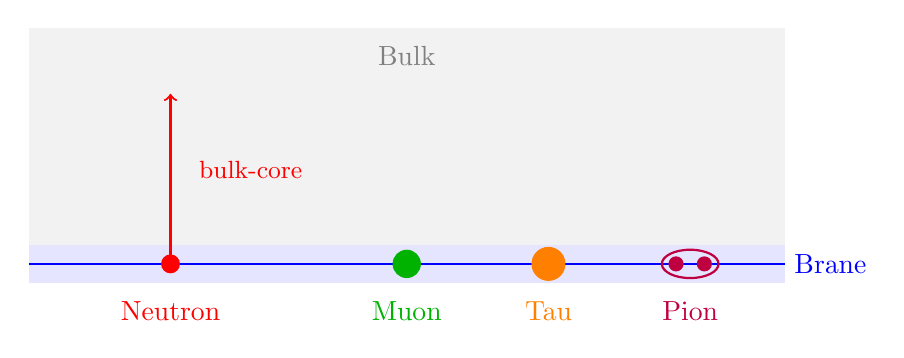
\begin{tikzpicture}[scale=1.2]
  % Brane
  \fill[blue!10] (-4,-0.2) rectangle (4,0.2);
  \draw[thick,blue] (-4,0) -- (4,0);
  \node[blue,right] at (4,0) {Brane};

  % Bulk region
  \fill[gray!10] (-4,0.2) rectangle (4,2.5);
  \node[gray] at (0,2.2) {Bulk};

  % Neutron (bulk-core)
  \draw[thick,red,->] (-2.5,0) -- (-2.5,1.8);
  \fill[red] (-2.5,0) circle (0.1);
  \node[red,below] at (-2.5,-0.3) {Neutron};
  \node[red,right] at (-2.3,1.0) {\small bulk-core};

  % Muon (brane-dominant)
  \fill[green!70!black] (0,0) circle (0.15);
  \node[green!70!black,below] at (0,-0.3) {Muon};

  % Tau (brane-dominant, higher mode)
  \fill[orange] (1.5,0) circle (0.18);
  \node[orange,below] at (1.5,-0.3) {Tau};

  % Pion (brane-dominant, composite)
  \draw[purple,thick] (3,0) ellipse (0.3 and 0.15);
  \fill[purple] (2.85,0) circle (0.08);
  \fill[purple] (3.15,0) circle (0.08);
  \node[purple,below] at (3,-0.3) {Pion};
\end{tikzpicture}
\caption{Ontological categories: bulk-core junction (neutron) vs.\ brane-dominant
excitations (muon, tau, pion). Circle size schematically indicates mode energy.}
\label{fig:ontology}
\end{figure}

% ==============================================================================
\section{The Neutron Anchor}
\label{sec:neutron}
% ==============================================================================

The neutron serves as the \textbf{anchor} of the Weak Program because:

\begin{enumerate}
  \item It is the only free-particle weak decay with all parameters measured
        to high precision
  \item Its bulk-core ontology provides the most stringent test of the 5D
        framework
  \item The NJSR (Neutron Junction Stability Radius) establishes the connection
        to nuclear binding
\end{enumerate}

\subsection{Key Results from Companion N}

Companion N establishes:

\begin{itemize}
  \item \textbf{Junction oscillation model} [P]: Neutron instability arises from
        oscillation modes of the bulk-core junction
  \item \textbf{Lifetime scaling} [P]/[OPEN]: Qualitative connection to junction
        geometry (numerical derivation flagged [OPEN])
  \item \textbf{Nuclear stabilization mechanism} [P]: Binding in nuclei modifies
        junction boundary conditions, stabilizing the neutron
\end{itemize}

\subsection{Reference}

The neutron junction model is grounded in Paper 3 (NJSR):
\begin{quote}
\textit{Neutron Lifetime from 5D Membrane Cosmology}\\
DOI: 10.5281/zenodo.18262721
\end{quote}

% ==============================================================================
\section{Lepton Spectrum Tomography: Muon and Tau}
\label{sec:leptons}
% ==============================================================================

Companions M and T extend the pipeline to purely leptonic decays, testing
whether brane-dominant configurations follow the same absorption → dissipation
→ release structure.

\subsection{Muon Decay (Companion M)}

The muon decay $\mu^- \to e^- \bar{\nu}_e \nu_\mu$ provides:

\begin{itemize}
  \item \textbf{Clean test case}: No hadronic complications
  \item \textbf{Same pipeline}: Absorption → Dissipation → Release applies
  \item \textbf{Mode index hypothesis}: $n_\mu > n_e$ explains mass hierarchy [P]/[OPEN]
\end{itemize}

Key equation (from Companion M):
\begin{equation}
\mathcal{A}_{\mu^-} = \{(e^-, \bar{\nu}_e, \nu_\mu)\}
\end{equation}
where $\mathcal{A}_{\mu^-}$ is the allowed output set [Dc].

\subsection{Tau Decay (Companion T)}

The tau provides a \textbf{mode-spectrum test}: if muon and tau share the same
ontology (brane-dominant), the pipeline should generalize without modification.

\begin{itemize}
  \item \textbf{Generalization confirmed}: Same pipeline structure
  \item \textbf{Mode index ordering}: $n_e < n_\mu < n_\tau$ [P]/[Def]
  \item \textbf{Near-equal BR}: BR($\tau \to e$) $\approx$ BR($\tau \to \mu$)
        explained by mode-spectrum overlap [P]/[OPEN]
\end{itemize}

\subsection{The Chiral Filter}

Both companions invoke a \textbf{chiral filter} $\mathcal{P}_{\mathrm{chir}}$
that enforces helicity constraints. This filter is:

\begin{itemize}
  \item \textbf{Universal hypothesis} [P]/[OPEN]: Same mechanism for all
        brane-dominant decays
  \item \textbf{Not derived from BC}: Derivation from boundary conditions
        remains [OPEN]
\end{itemize}

% ==============================================================================
\section{The Pion Bridge: Hadron → Lepton Injection Test}
\label{sec:pion}
% ==============================================================================

Companion P addresses the first \textbf{hadron → lepton} transition in the
program, testing whether the pipeline extends from leptonic to hadronic
initial states.

\subsection{Pion Ontology}

The charged pion $\pi^+$ is modeled as:

\begin{postulate}[Pion as Brane-Dominant Composite {\normalfont [P]}]
\label{post:pion}
The $\pi^+$ is a brane-layer bound state of constituent quarks, with
energy predominantly localized on the brane.
\end{postulate}

\textbf{Note:} This is a postulate, not a derivation. The specific micro-ontology
(junction-pair, etc.) is flagged [P]/[OPEN] as a candidate only.

\subsection{Helicity Suppression}

The dominant feature of pion leptonic decay is helicity suppression:
\begin{equation}
\Gamma(\pi^+ \to \ell^+ \nu_\ell) \propto m_\ell^2
  \left(1 - \frac{m_\ell^2}{m_\pi^2}\right)^2
\end{equation}

\begin{tcolorbox}[edcGuardrail, title={Epistemic Status: Helicity Suppression}]
The $m_\ell^2$ scaling is a \textbf{baseline fact} [BL] from SM/PDG.
Companion P does \textbf{not} derive this scaling from EDC boundary conditions.
The derivation is flagged [OPEN].
\end{tcolorbox}

\subsection{What Companion P Establishes}

\begin{itemize}
  \item \textbf{Pipeline unity}: Same absorption → dissipation → release
        structure applies to composite hadrons
  \item \textbf{Ontological consistency}: Brane-dominant composite is
        consistent with leptonic output selection
  \item \textbf{Allowed output set}: $\mathcal{A}_{\pi^+} = \{(\mu^+, \nu_\mu),
        (e^+, \nu_e)\}$ [Dc]
\end{itemize}

\subsection{What Companion P Does NOT Claim}

Companion P explicitly avoids:

\begin{itemize}
  \item Derivation of $m_\pi = 140$ MeV from first principles [OPEN]
  \item Derivation of $\tau_\pi = 26$ ns from first principles [OPEN]
  \item Derivation of BR ratio from EDC (helicity suppression = [BL])
  \item Explanation of quark confinement in 5D [OPEN]
\end{itemize}

% ==============================================================================
\section{Consolidated Knowledge Status}
\label{sec:status}
% ==============================================================================

\subsection{What We Know Now}

Table~\ref{tab:know} summarizes established results across the Weak Program.

\begin{table}[h]
\centering
\caption{Established results in the EDC Weak Program}
\label{tab:know}
\begin{tabular}{lll}
\toprule
\textbf{Result} & \textbf{Tag} & \textbf{Source} \\
\midrule
Unified pipeline structure & [Def] & All companions \\
Bulk-core vs.\ brane-dominant distinction & [P] & N vs.\ M/T/P \\
Allowed output sets & [Dc] & Conservation laws \\
Frozen projection operator form & [Def] & Companion H \\
Suppressed bulk leakage & [P] & All companions \\
\bottomrule
\end{tabular}
\end{table}

\subsection{What Remains Truly OPEN}

Table~\ref{tab:open} consolidates open problems from all companions.

\begin{longtable}{llp{6cm}}
\caption{Consolidated open problems}
\label{tab:open} \\
\toprule
\textbf{ID} & \textbf{Particle} & \textbf{Problem} \\
\midrule
\endfirsthead
\toprule
\textbf{ID} & \textbf{Particle} & \textbf{Problem} \\
\midrule
\endhead
OPEN-N1 & Neutron & Derive $\tau_n$ from junction geometry \\
OPEN-N2 & Neutron & Quantify nuclear stabilization mechanism \\
OPEN-N3 & Neutron & Derive $G_F$ from 5D coupling \\
\midrule
OPEN-M1 & Muon & Derive $\mathcal{P}_{\mathrm{chir}}$ from BC \\
OPEN-M2 & Muon & Derive $\tau_\mu$ from first principles \\
OPEN-M3 & Muon & Quantify mode index $n_\mu$ \\
\midrule
OPEN-T1 & Tau & Explain BR($e$) $\approx$ BR($\mu$) quantitatively \\
OPEN-T2 & Tau & Hadronic tau decays \\
OPEN-T3 & Tau & Derive $\tau_\tau$ from first principles \\
\midrule
OPEN-P1 & Pion & Derive $m_\pi$ from 5D binding \\
OPEN-P2 & Pion & Derive $\tau_\pi$ from first principles \\
OPEN-P3 & Pion & Derive $m_\ell^2$ scaling from BC \\
OPEN-P4 & Pion & Junction-pair micro-ontology validation \\
OPEN-P5 & Pion & Neutral pion $\pi^0 \to \gamma\gamma$ \\
\bottomrule
\end{longtable}

% ==============================================================================
\section{Falsifiability and Non-Overclaim Canon}
\label{sec:falsifiability}
% ==============================================================================

\subsection{Structural Falsifiability}

Each companion specifies conditions under which its claims would fail.
The Weak Program as a whole is falsifiable if:

\begin{enumerate}
  \item \textbf{Pipeline fails for any particle}: A decay is discovered that
        cannot be mapped to absorption → dissipation → release
  \item \textbf{Ontology fails}: A bulk-core particle behaves as brane-dominant
        or vice versa
  \item \textbf{Selection rules fail}: Forbidden channels dominate observed
        branching ratios
  \item \textbf{Universality fails}: Different particles require fundamentally
        different chiral filters
  \item \textbf{Conservation fails}: Energy/momentum ledgers do not close
\end{enumerate}

\subsection{Non-Overclaim Canon}

\begin{tcolorbox}[edcGuardrail, title={Non-Overclaim Statement}]
The EDC Weak Program does \textbf{NOT} claim:
\begin{itemize}
  \item Derivation of particle masses from first principles
  \item Derivation of lifetimes from first principles
  \item Derivation of branching ratios beyond selection-rule constraints
  \item Explanation of CP violation
  \item Resolution of the strong CP problem
  \item Unification with gravity beyond Framework v2.0
\end{itemize}
All numerical values in the companions are either [BL] (PDG/CODATA) or
explicitly flagged [OPEN].
\end{tcolorbox}

\subsection{Epistemic Discipline}

The Weak Program adheres to strict epistemic tagging:

\begin{table}[h]
\centering
\caption{Epistemic tag definitions}
\label{tab:tags}
\begin{tabular}{ll}
\toprule
\textbf{Tag} & \textbf{Meaning} \\
\midrule
{[BL]} & Baseline fact from SM/PDG/CODATA \\
{[Def]} & Definition (conventional) \\
{[Dc]} & Deduced/constrained from definitions + conservation \\
{[P]} & Postulate (EDC-specific hypothesis) \\
{[Der]} & Derived (explicit proof chain exists) \\
{[OPEN]} & Unresolved—flagged for future work \\
\bottomrule
\end{tabular}
\end{table}

% ==============================================================================
\section{Practical Reader Guide}
\label{sec:guide}
% ==============================================================================

\subsection{Recommended Reading Order}

For readers new to the EDC Weak Program:

\begin{enumerate}
  \item \textbf{Framework v2.0} (DOI: 10.5281/zenodo.18299085)\\
        Establishes 5D foundation, bulk–brane conservation, canonical notation

  \item \textbf{Companion H} (DOI: 10.5281/zenodo.18307539)\\
        Thick-brane microphysics foundation

  \item \textbf{Paper 3 / NJSR} (DOI: 10.5281/zenodo.18262721)\\
        Neutron junction model—the anchor result

  \item \textbf{Companion N}\\
        Neutron decay in full pipeline framework

  \item \textbf{Companion M}\\
        Muon decay—first brane-dominant test

  \item \textbf{Companion T}\\
        Tau decay—mode-spectrum generalization

  \item \textbf{Companion P}\\
        Pion decay—hadron → lepton bridge
\end{enumerate}

\subsection{Quick Reference: Where to Find What}

\begin{table}[h]
\centering
\caption{Topic locator}
\label{tab:locator}
\begin{tabular}{ll}
\toprule
\textbf{Topic} & \textbf{Document} \\
\midrule
Bulk–brane conservation & Framework v2.0, Remark 4.5 \\
Frozen projection definition & Companion H, §4 \\
Junction oscillation model & Paper 3, §5; Companion N \\
Mode index hypothesis & Companion M, §2; Companion T, §2 \\
Helicity suppression (EDC view) & Companion P, §5 \\
Selection rules derivation & Companion F \\
Gauge emergence & Companion G \\
\bottomrule
\end{tabular}
\end{table}

\subsection{Dependency Graph}

Figure~\ref{fig:deps} shows the logical dependencies among Weak Program documents.

\begin{figure}[h]
\centering
\begin{tikzpicture}[
  node distance=1.5cm,
  doc/.style={rectangle, draw, rounded corners, minimum width=2.5cm, minimum height=0.8cm},
  arrow/.style={->, thick}
]
  % Foundation layer
  \node[doc] (fw) {Framework v2.0};

  % Second layer
  \node[doc, below left=1cm and 0.5cm of fw] (H) {Companion H};
  \node[doc, below right=1cm and 0.5cm of fw] (p3) {Paper 3};

  % Third layer
  \node[doc, below=1cm of H] (F) {Companion F};
  \node[doc, below=1cm of p3] (N) {Companion N};

  % Fourth layer
  \node[doc, below left=1cm and -0.5cm of N] (M) {Companion M};
  \node[doc, below=1cm of N] (T) {Companion T};
  \node[doc, below right=1cm and -0.5cm of N] (P) {Companion P};

  % Arrows
  \draw[arrow] (fw) -- (H);
  \draw[arrow] (fw) -- (p3);
  \draw[arrow] (H) -- (F);
  \draw[arrow] (H) -- (N);
  \draw[arrow] (p3) -- (N);
  \draw[arrow] (N) -- (M);
  \draw[arrow] (N) -- (T);
  \draw[arrow] (N) -- (P);
  \draw[arrow] (M) -- (T);
  \draw[arrow] (T) -- (P);
\end{tikzpicture}
\caption{Document dependencies in the EDC Weak Program. Arrows indicate
``builds upon'' relationships.}
\label{fig:deps}
\end{figure}

% ==============================================================================
\section{Conclusion}
\label{sec:conclusion}
% ==============================================================================

The EDC Weak Program demonstrates that a single conceptual framework—based on
thick-brane microphysics with a unified absorption → dissipation → release
pipeline—can accommodate weak decays across:

\begin{itemize}
  \item \textbf{Bulk-core} configurations (neutron)
  \item \textbf{Brane-dominant fundamental} excitations (muon, tau)
  \item \textbf{Brane-dominant composite} bound states (pion)
\end{itemize}

The program is characterized by:

\begin{enumerate}
  \item \textbf{Ontological clarity}: Explicit distinction between particle types
  \item \textbf{Epistemic discipline}: Rigorous tagging of claims
  \item \textbf{Falsifiability}: Explicit failure conditions
  \item \textbf{Honest scope}: Clear registry of open problems
\end{enumerate}

This overview consolidates the program's current state without introducing
new claims. All technical content refers to source documents archived with
DOIs, ensuring reproducibility and auditability.

\subsection{Program Status Summary}

\begin{table}[h]
\centering
\caption{EDC Weak Program completion status}
\label{tab:status}
\begin{tabular}{llll}
\toprule
\textbf{Companion} & \textbf{Particle} & \textbf{Version} & \textbf{Ontology} \\
\midrule
N & Neutron & v3.0 & Bulk-core junction \\
M & Muon & v0.2 & Brane-dominant (fundamental) \\
T & Tau & v0.1 & Brane-dominant (higher mode) \\
P & Pion & v0.3 & Brane-dominant (composite) \\
\bottomrule
\end{tabular}
\end{table}

\vspace{1em}
\begin{center}
\rule{0.5\textwidth}{0.4pt}
\end{center}
\vspace{0.5em}

\noindent\textit{Document version: 1.0}\\
\textit{Generated: January 2026}\\
\textit{This is an umbrella document; it references but does not modify
archived companions.}

% ==============================================================================
\end{document}
% ==============================================================================
